\documentclass[a4paper, 11pt, final, garamond]{book}
\usepackage{cours-preambule}

\makeatletter
\renewcommand{\@chapapp}{Devoir surveill\'e -- num\'ero}
\makeatother

\begin{document}
\setcounter{chapter}{8}

\def\lspace{25}

\chapter{Commentaires sur le DS n\degree09}
\section{Commentaires généraux}

Gloablement, les bases ne sont pas solides, et on retrouve la même dynamique que
pour le DS précédent~: vous saviez faire des $E-\pH$ mais pas des acide-base…
Ici, \textsc{Stirling} a été bien réussi puisque c'était un des exercices de
l'année dernière, mais clairement cette expérience montre que vous apprenez sans
comprendre (et je ne la retenterai plus~!). L'exercice 1 appuie cette analyse,
puisque c'est un exercice d'équilibre thermodynamique très classique du chapitre
2 (avec quelques éléments des chapitres 3 et 4). \textbf{Il faudra absolument
	revoir la base}.

\begin{center}
	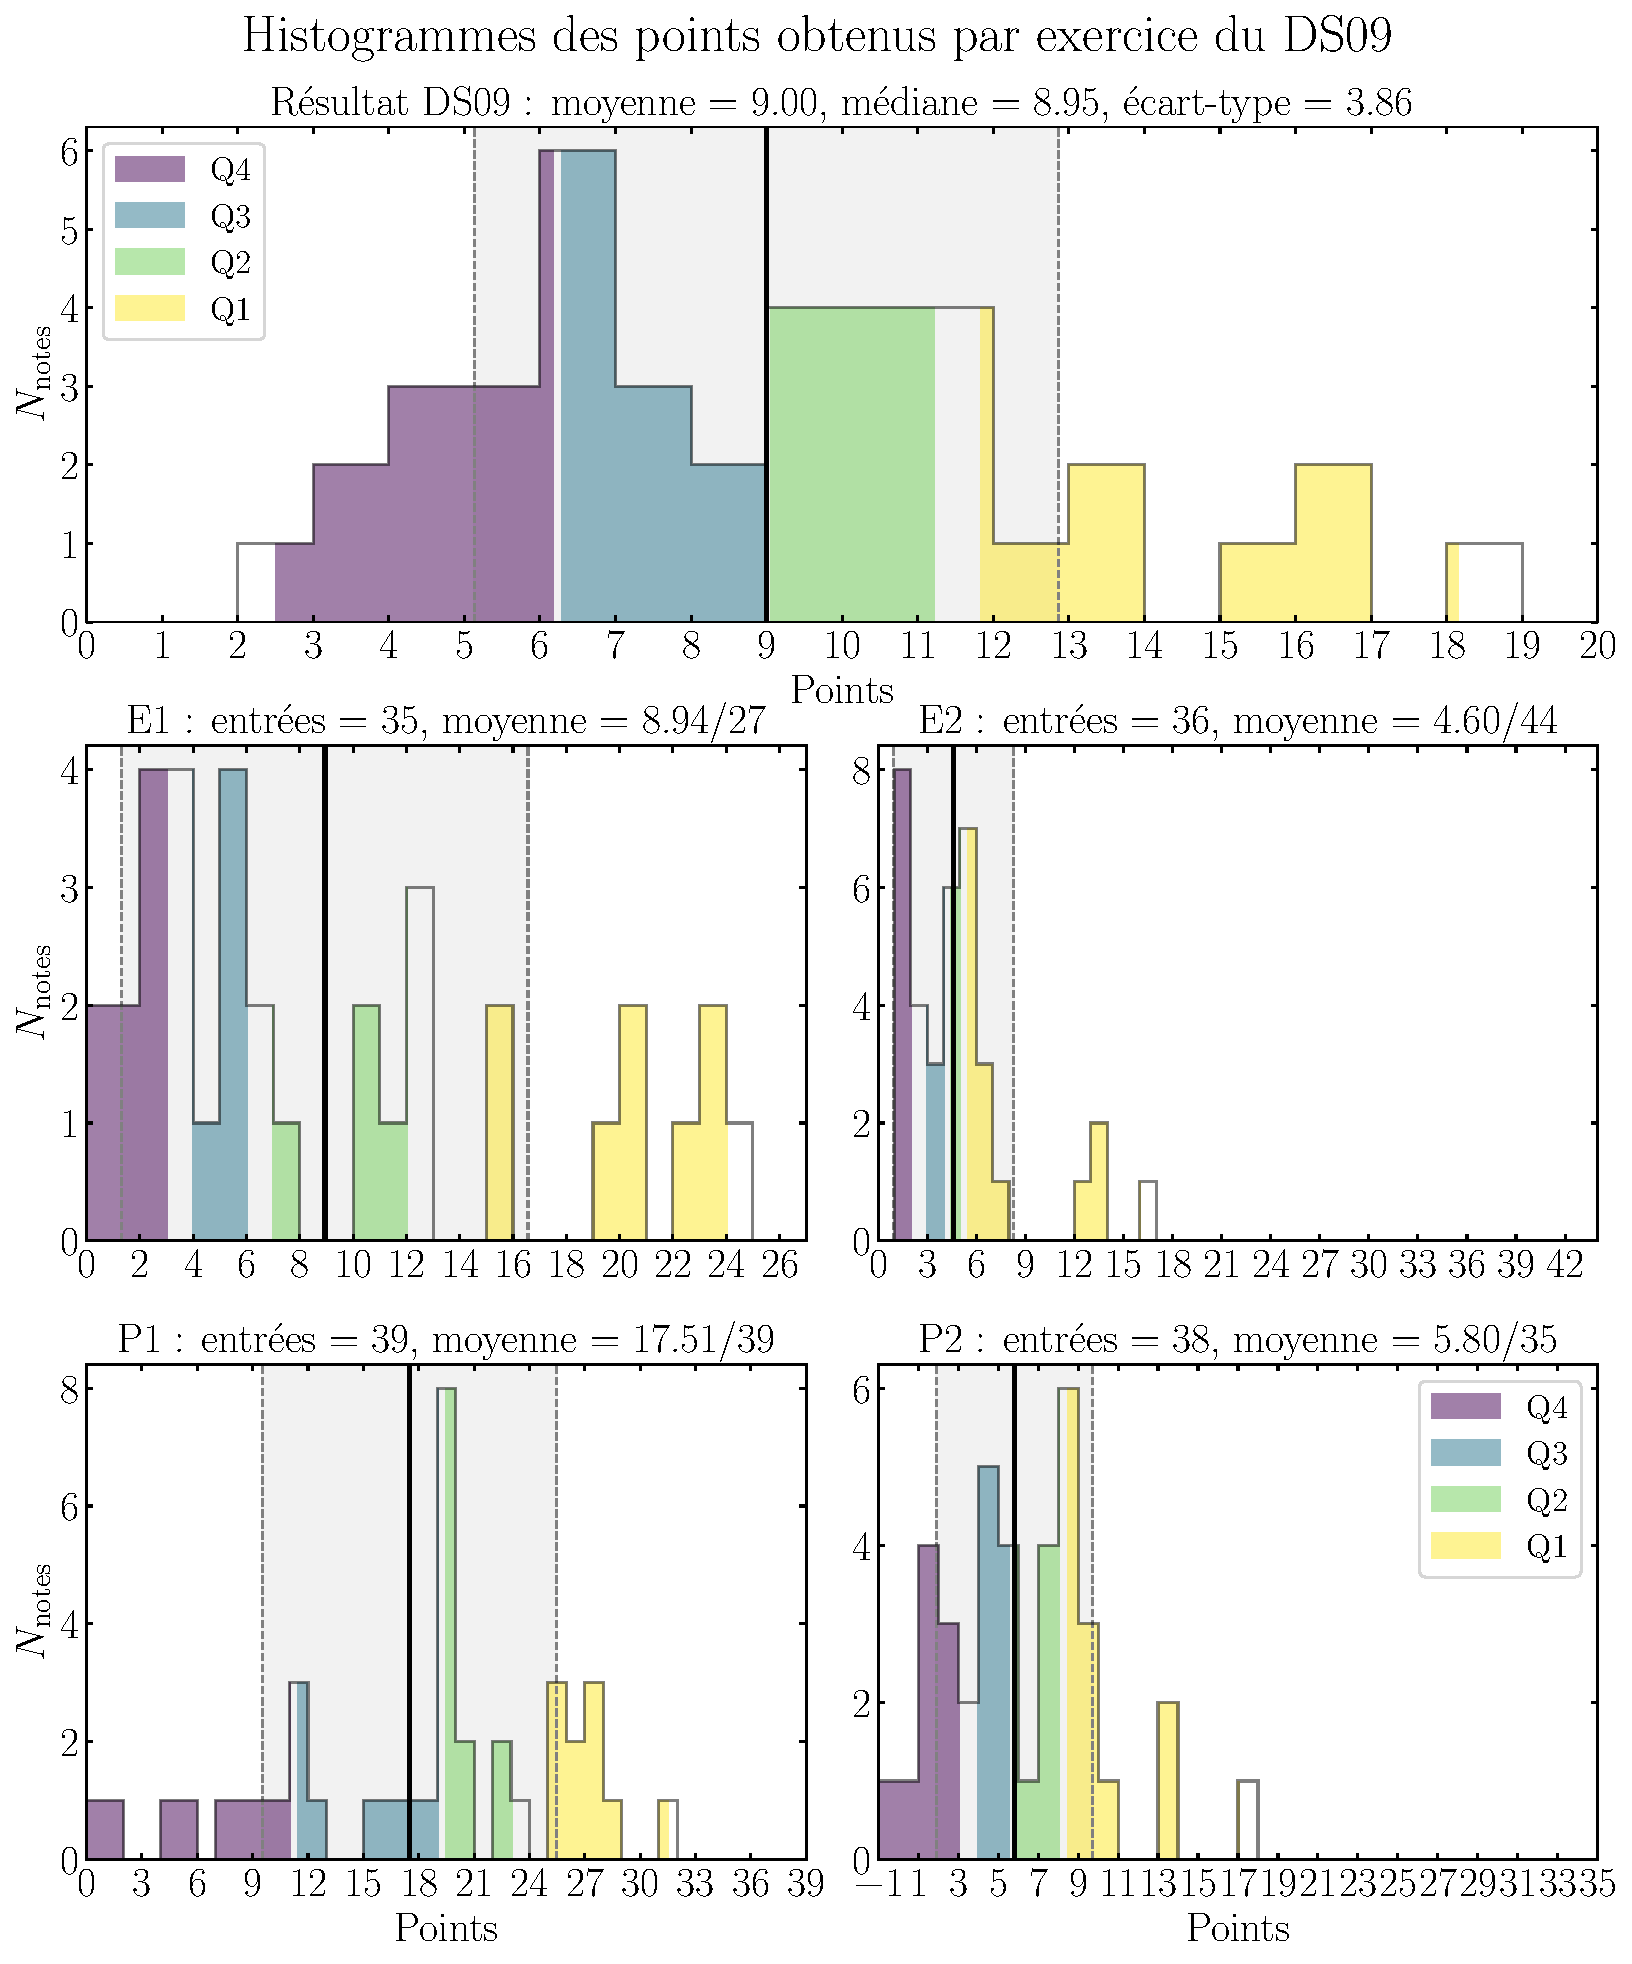
\includegraphics[width=.9\linewidth]{DS09_hist_all}
\end{center}

Je suis d'avis que la thermodynamique fait partie de ces disciplines qui sont
\textit{vraiment} de la Physique belle et pure, pleine d'analyse, de
modélisation et d'intuition, et la diffère très bien des disciplines plus
mathématiques comme la mécanique ou des sciences de l'ingénieur comme peut
l'être l'électrocinétique. Bref, je divague, mais comprendre la thermodynamique
c'est un signe non négligeable de bonne maîtrise de la
Physique\ftn{\textbf{Attention}, je ne dis pas que si vous n'avez pas réussi ce
	DS vous ne maîtrisez pas la physique~; encore une fois un DS c'est un test à
	un instant $t$ sur une partie à peine finie. Je veux surtout dire que si vous
	voulez vous améliorer en Physique, comprendre la thermodynamique est un bon
	moyen~!}.

\begin{tcn}(prop)"bomb"{Attention}
	\begin{itemize}
		\item Numérotez les annexes~!
		\item Écrivez le numéro de la question qui amène à
		      l'annexe~!!
		\item Vous ne pouvez \textbf{pas donner les expressions des rendements
			      en valeurs absolues}~: il faut connaître le signe des échange et les
		      écrire directement, sinon vous vous rajoutez une difficulté à les
		      déterminer.
		\item Un rendement de 1 ça n'existe \textbf{pas} pour les machines
		      thermiques, même \textbf{théoriquement} à cause du second principe~!!
	\end{itemize}
\end{tcn}

\setcounter{section}{0}
\section[27]"E"{Étude de deux gaz parfaits dans un cylindre}
Exercice classique de début de thermodynamique, basé sur l'équilibre,
\textbf{très mal réussi}. N'inventez pas des résultats (comme «~c'est
isobare~»).
\bigbreak
\textbf{Attention}, dans ce genre d'énoncé de concours très commun dans les
petits concours, il faut justifier la réponse \textbf{sans raisonnement par
	l'absurde ou par élimination}. Vous devez \textbf{démontrer complètement} le
résultat.
\bigbreak
\textbf{Il faut indiquer clairement la (ou les) lettre(s) correspondant à la
	réponse~!}
\begin{enumerate}[label=\sqenumi]
	\item[n]{7} % Q1
	Question de base de TD sur les équilibres thermodynamiques… très mal
	réussie. J'ai vu des sommes de températures…~! \textbf{$T$ est une grandeur
		intensive~!}
	\item[n]{2} % Q2
	La température initiale était $T_0$, pas $T$. C'était à déduire puisqu'il y a
	équilibre thermodynamique initial, or $(2)$ contact thermostat à $T_0$.
	\item[n]{5} % Q3
	La plupart d'entre vous a complètement ignoré l'extensivité de $U$ et a fait
	des $\Delta{U}$ sans distinguer $\Delta{U}_1$ et $\Delta{U}_2$. Très gros
	manque de maîtrise à ce niveau-là.
	\item[n]{7} % Q4
	Il faut écrire la définition avec $P\ind{ext}$, et clairement justifier
	pourquoi $P = P\ind{ext}$. De même, avoir $T_2 = T_0$ n'est pas équivalent à
	une transformation isotherme, il faut écrire $\boxed{T = T_0}$~! De même,
	écrire le premier principe en entier $\Delta{U}_2 = W_2 + Q_2$.
	\begin{center}
		\LARGE
		$P\ind{ext} = P_2$ est simplement \textbf{faux}, puisque $P$ varie avec la
		température~! $P_2$ est une constante~! C'est $P = P\ind{ext}$~!!
	\end{center}
	\olditem[\fbox{5-6}] % Q5
	RAS.
\end{enumerate}

\section[44]"E"{Cycle de \textsc{Carnot}}
Un exercice qui vous a pas mal bloqué-es. Il sera intéressant à reprendre à tête
reposée.
\begin{enumerate}[label=\sqenumi]
	\item[n]{3} % Q1
	Répondre à la partie sur le cycle. \textbf{Beaucoup ne savent pas dire quel
		est le second principe}~!! C'est grave et triste vu son importance dans le
	fonctionnement même du monde naturel.
	\item[n]{5} % Q2
	Le cycle est \textbf{réversible}, donc chacune des transformations doit
	l'être. De plus, même si vous ne le connaissez pas, un diagramme $(X,Y)$ a $X$
	en ordonnée et $S$ en abscisse~! \textbf{Attention} la correction de base
	avait le cycle dans le mauvais sens. Vous trouverez sur \textbf{Cahier de
		Prépa} la page avec le bon sens.
	\item[n]{4} % Q3
	Ne partez pas dans des calculs à rallonge pour déterminer le rendement de
	\textsc{Carnot}~: c'est la démonstration en 3 lignes du cours en ayant
	$\frac{Q_C}{T_C} + \frac{Q_F}{T_F} = 0$, puisqu'alors $S\ind{cr} = 0$…
	\textbf{Bilan d'énergie $\equiv$ 1\ier{} ppe.}, et \textbf{bilan d'entropie
		$\equiv$ 2\up{d} ppe.}~!
	\item[n]{4} % Q4
	Très peu traitée.
	\item[n]{4} % Q5
	Bien lire l'énoncé~: l'état 1 correspond au moment \textbf{juste avant la
		phase de compression adiabatique}. De plus, la machine de \textsc{Carnot}
	étant réversible, il faut que \textbf{chaque étape soit réversible}, donc
	les adiabatiques et les isothermes doivent être indiquées comme étant
	réversibles.
	\item[n]{5} % Q6
	Il faut séparer les deux variables, puis «~différencier des deux côtés~»,
	selon $P$ d'une part et selon $V$ d'autre part.
	\olditem[\fbox{7-11}] % Q7-11
	RAS, non traitées.
	% \item[n]{2} % Q7
	% \item[n]{5} % Q8
	% \item[n]{5} % Q9
	% \item[n]{4} % Q10
	% \item[n]{2} % Q11
\end{enumerate}

\setcounter{section}{0}
\section[39]"P"{Moteur de \textsc{Stirling}}
Un exercice qui vous a bien fait plaisir puisque c'était le même que celui de
l'année dernière. Il n'est cependant jamais réussi en totalité, et souvent
survolé ou bâclé~: faites attention aux signes, et détaillez les étapes de
calcul pour le premier travail calculé. Il faut intégrer le fait que $Q_C$ sont
tous les $Q$ qui vérifient le signe de la machine, ici $Q_C = \sum Q_i$ avec
$Q_i > 0$.
\smallbreak
Les résultats sont remarquablement centrés autour de 19/39 par ailleurs.
\begin{enumerate}[label=\sqenumi]
	\item[n]{6} % Q1
	Pensez à justifier le signe de $W$ par l'étude des aires relatives.
	\item[n]{4} % Q2
	\textbf{Indiquez que vous avez répondu à la question sur l'annexe}, ou
	\textit{a minima} écrire le numéro de la question sur la copie. Possible
	malus Q. Il faut \textbf{indiquer le sens de parcours}.
	\item[n]{8} % Q3
	Il faut écrire $W = -\int P\ind{ext}\dd{V}$ et bien justifier toutes les
	étapes du calcul.
	\smallbreak
	Une démonstration qui utilise les expressions de $\Delta{S}$ qui sont
	hors programme, mais très bien réalisée~!
	\item[n]{3} % Q4
	Bien.
	\item[n]{3} % Q5
	Beaucoup de problèmes de signes dans ces questions-là. Ne vous précipitez pas
	en disant «~de même qu'en Q3~» pour vous tromper de signe ensuite.
	\item[n]{2} % Q6
	RAS
	\item[n]{3} % Q7
	\textbf{Rendement idéal $\neq$ rendement réel}~: il y a le rendement réel
	(ellipse), le rendement idéal (cycle idéalisé), et le rendement de
	\textsc{Carnot} (réversible).
	\smallbreak
	$W$ dans les rendements/efficacités, c'est \textbf{toujours $W\ind{cycle}$},
	puisqu'il n'y a qu'une seule sorte de travail fait par un seul système~; on ne
	choisit pas que $W_{34}$ parce qu'il est négatif.
	\item[n]{5} % Q8
	Idem, le rendement de \textsc{Carnot} n'est pas le rendement idéal d'une
	machine, c'est le \textbf{rendement maximal d'une machine idéale}~!
	\item[n]{3} % Q9
	Un \textbf{rendement de 1 ça doit vous choquer} pour les machines dithermes~!
	Par essence on a «~besoin~» de perdre de l'énergie pour que la machine
	fonctionne…
	\item[n]{2} % Q10
	Attention, températures en \textbf{kelvins} \si{K}~!
\end{enumerate}

\section[35]"P"{Étude thermodynamique d'une chambre froide}
Un début correct pour la plupart, mais il y a trop d'entre vous qui n'ont rien
retenu du chapitre concerné. Les transferts sont dans le mauvais sens, pas
justifiés ou mal justifiés, et l'efficacité est mal écrite (voir définie comme
$\frac{\text{perte}}{\text{coût}}$)~!
\smallbreak
À partir de la Q6 l'exercice devient intéressant, mais les cycles ont été mal
faits. \textbf{Travaillez sur la lecture des échelles logarithmiques}, et
reprenez le tracé de cet exercice.
\begin{enumerate}[label=\sqenumi]
	\item[n]{3} % Q1
	Quelques super réponses~! Le frigo vu en TP a bien servi.
	\item[n]{3} % Q2
	Il faut correctement \textbf{justifier les signes}~! On veut refroidir la
	source froide, donc on en reçoit de la chaleur~: $Q_F > 0$. On veut
	réchauffer la source chaude, donc on y donne de la chaleur~: $Q_C < 0$. Ce
	transfert est opposé au sens d'évolution spontané des transferts de chaleur,
	donc cela nous coûte un travail~: $W > 0$.
	\item[n]{1} % Q3
	RAS.
	\item[n]{5} % Q4
	\textbf{Si une machine est réversible, on a l'\xul{égalité} de
		\textsc{Clausius}}~! \xul{Démontrer} les deux équations des machines avec le
	premier et le second principe.
	\item[n]{2} % Q5
	      {\Large L'unité naturelle des températures c'est les \textbf{kelvins}~!!}
	\smallbreak
	Attention aux chiffres significatifs~! Les \num{273.15} ne sauraient ajouter
	de la précision aux données qui sont de \SI{45}{\degreeCelsius} et
	\SI{3}{\degreeCelsius}.
	\item[n]{2} % Q6
	Quelques tentatives de cycle, c'est bien~! Attention à la lecture des
	échelles logarithmique cependant~: au-dessus de $10^1$, ça n'est pas $11$
	mais $20$~! Vérifiez vos placements avec les isothermes.
	\bigbreak
	\textbf{Attention} le corrigé est très, très faux dans le tracé du cycle. Vous
	trouverez sur \textbf{Cahier de Prépa} la page avec le bon cycle.
	\olditem[\fbox{7-14}] % Q7
	RAS, globalement non fait puisque dépendant du cycle, mais c'est dommage.
	Question 9 très mal comprise.
	% \item[n]{2} % Q8
	% \item[n]{4} % Q9
	% \item[n]{2} % Q10
	% \item[n]{2} % Q11
	% \item[n]{3} % Q12
	% \item[n]{2} % Q13
	% \item[n]{2} % Q14
\end{enumerate}

\end{document}
